%!TEX root = ../thesis.tex
%*******************************************************************************
%****************************** Seventh Chapter **********************************
%*******************************************************************************

\chapter{Homeostasis Optimisation}

\section[Optimisation Motivations]{Optimisation Motivations}

\subsection[Analogue Hardware Challenges]{Analogue Hardware Challenges}

\noindent Novel computer hardware solutions that employ analogue devices still exhibit limited precision and unreliability. However, both physical and algorithmic techniques can be employed to mitigate these issues. In contrast to digital technology, the analogue approach inherently involves a degree of imprecision. \\

\noindent Analogue devices, such as RRAM, are susceptible to a number of issues, including stuck states, device-to-device variability and I-V nonlinearity. However, the development of advanced fabrication methods and circuit-level optimisations has enabled the mitigation of some of these non-idealities, while algorithmic techniques have also been shown to be effective in reducing their impact.\\

\noindent In contrast to the digital paradigm, where a multitude of physical imperfections are effectively concealed within a bit representation (either '1' or '0'), analogue electronics is confronted with significant challenges due to the intrinsic imprecision associated with non-discrete systems. Even with a minimal amount of non-idealities, it is challenging to encode information with perfect precision using an exact conductance value.\\

\noindent However, non-idealities do exist and can result in significant deviations from ideal behaviour. These include the device becoming stuck in certain conductance states, undergoing changes in conductance over time, showing non-linear current-voltage characteristics, or displaying non-linear conductance modulation in response to voltage stimuli. \\

\noindent It could be argued that analogue computing's more fundamental challenge lies in its reduced precision compared to digital computing, especially when digital systems utilise 16 or more bits of representation. While these issues may be grounds for disqualification in many applications, this may not be the case for machine learning applications, which often employ reduced precision computing, even within digital systems. \\

\noindent In general, machine learning models demonstrate a degree of robustness to minor alterations, such as the presence of noise \cite{cheney2017robustness}. In the event of significant deviations from ideal conditions, hardware imperfections may result in a decline in accuracy. However, this does not necessarily render the system inoperable. It is, therefore, crucial to comprehend the impact of non-idealities and to ascertain how they can be effectively mitigated. \\

\noindent In the context of linear algebra applications, a proportional relationship between voltage and current (i.e. Ohmic behaviour) is the preferred option. This is due to the fact that Ohm's law is employed in the implementation of multiplication, as previously discussed. Nevertheless, exceptions to this linear relationship do arise, particularly in the case of high-resistance devices \cite{mehonic2017intrinsic}. \\

\noindent A number of approaches exist at the device and circuit level that facilitate the resolution or even circumvention of the issue of nonlinearity. During the fabrication of RRAM devices, the adoption of a hot-forming step can result in the generation of more linear characteristics \cite{sung2018effect}. \\

\noindent In the case of individual device programming, the adoption of a transistor-to-resistor ratio (1T1R) architecture can facilitate the precise tuning of memristor conductance, despite the presence of any I-V nonlinearities \cite{li2018analogue}. Alternatively, a charge-based accumulation approach can be employed, wherein a constant voltage is applied, but the input is encoded into pulse width \cite{amirsoleimani2020memory}. This eliminates the dependence on the shape of the I-V curve. \\

\noindent It is possible that some memristive devices may become fixed in a specific conductance state. This phenomenon has been observed following processes such as electroforming, as well as after several successful programming cycles \cite{joksas2022nonideality}. In general, the greater the discrepancy between the intended and actual conductance, the greater the potential for adverse effects. Therefore, it is of paramount importance to identify methods for the prevention or mitigation of faulty devices.\\

\noindent The overall effect of a device becoming stuck is contingent upon the behaviour of other devices, and thus this phenomenon can be employed to mitigate the negative effects. To illustrate, if a device becomes stuck, its negative effect may be counteracted by adjusting the conductance of another device in the differential pair \cite{liu2017rescuing}. On occasion, such an adjustment may occur accidentally, whereby both devices in a differential pair become stuck simultaneously.\\

\noindent As an alternative, if faulty devices can be identified prior to programming, more sophisticated mapping strategies can be employed. The most significant weights can be mapped onto crossbar rows and columns with the lowest incidence of stuck devices \cite{gaol2021reliable}. The most significant terms refer to the weights that could have the greatest impact on accuracy. One way to identify such weights is to calculate of sensitivity $\Delta w_{i,j} := - \eta \frac{\partial E}{\partial \Delta w_{i,j}}$, for each weight $w_{i,j}$, where \textit{E} is the back-propagated loss at the current neuron and $\eta$ is the learning rate.\\

\noindent The term 'limited dynamic range nonideality' is used to describe a situation whereby the $\frac{G_{on}}{G_{off}}$ ratio is relatively small, which can ultimately result in a reduction in effective precision. In the context of other non-idealities, such as device variability, limited dynamic range can result in a reduction in the number of distinguishable states that are available. \\

\noindent If each state is associated with a certain amount of absolute variability, it is evident that a larger dynamic range is preferable, as it allows for a more effective differentiation between those states that are less distinct. The impact of the dynamic range is highly dependent on the specific application. Should one desire to utilise analogue arrays for the storage of digital information, an enhanced dynamic range will facilitate a greater precision in the number of equivalent bits.\\

\noindent Nevertheless, when considering the acceleration of linear algebra operations (and, by extension, machine learning), such comparisons cannot be made with the same degree of ease. As these hardware accelerators are based on analogue computation, the concept of 'bits' – although potentially useful – does not apply directly. In analogue contexts, an error is defined as any deviation from the intended value. The magnitude of the error is the key factor in determining the severity of the mistake. \\

\noindent In the context of inference applications, a large dynamic range is not a crucial factor. If a naive mapping scheme is employed whereby the value of a weight is represented using a single conductance value, then the inaccuracies produced by this imperfect mapping can be addressed with a $\frac{G_{on}}{G_{off}}$ ratio of as low as 3 \cite{mehonic2019simulation}. In other contexts, the impact of limited dynamic range cannot be evaluated without first understanding the nature of other non-idealities, namely the deviations they cause.\\

\noindent Line resistance represents a non-ideality that arises from the presence of non-zero interconnect resistances in crossbar arrays. In the event of its presence, this results in discrepancies from the ideal computation of vector-matrix products. While the impact on accuracy can be significant, there are both physical and algorithmic techniques that can be employed to mitigate it. \\

\noindent One of the most straightforward methods for mitigating the impact of line resistance is to enhance the ratio between the resistance of the devices and the resistance of the interconnecting wires. As resistance is inversely proportional to the cross-sectional area of the wire, one method of reducing interconnect resistance is to increase the width of the wires \cite{li2017three}.\\

\noindent However, this can be challenging in dense arrays, and an alternative approach is to use more conductive materials, for example, $2nm$ platinum nanofins \cite{pi2019memristor}. Another approach is to increase the resistance of the crossbar devices, although this can sometimes result in less stable device behaviour. \\

\noindent At the circuit level, a variety of techniques may be employed which utilise the systematic properties of line resistance in different ways. For instance, a technique designated as double biasing can facilitate a more symmetrical distribution of electric potentials within crossbar arrays, thereby attenuating the impact of line resistance effects \cite{hu2016dot}. As the size of the crossbar array increases, voltage drops tend to accumulate. \\

\noindent Therefore, splitting up the array into smaller units \cite{xia2016technological}, or even organising them in three-dimensional structures \cite{xia2019memristive} can help to mitigate this issue. In considering the specific applications for which crossbar arrays are to be employed, algorithms may be deployed to ascertain optimal mappings from software parameters to physical quantities, such as voltage and conductance.  A nonlinear mapping from weights to conductances can be employed to counteract the detrimental effects of line resistance. \\

\noindent Alternatively, sensitivity analysis can identify the weights that are most sensitive, and thus map them closest to the applied voltages, where their contribution would be disturbed the least \cite{agrawal2019x}. In the specific context of supervised learning, input intensities may be predicted, and the inputs with the highest expected intensity (as well as the corresponding weights) can be mapped closest to the outputs in order to minimise the negative effects of line resistance. \\

\noindent When training networks directly on crossbar arrays, i.e. in situ, linear adjustments of conductance are the preferred approach \cite{burr2015experimental}. In order to ensure a linear response, the system must be modified physically. Some previous studies have proposed adjusting the device structure \cite{woo2016improved}, typically by introducing additional layers \cite{wu2018methodology}. An alternative approach is combining memristive devices with CMOS transistors, which help to improve the linearity \cite{ambrogio2018equivalent}.\\

\noindent Random telegraph noise (RTN) is defined as the occurrence of unpredictable switching between two or more discrete voltage levels in electronic devices \cite{puglisi2016guidelines}. This phenomenon is frequently observed in memristors. RTN is more commonly experienced in devices with higher resistance, which can impede the use of such devices for reducing power consumption or mitigating the effects of line resistance. To circumvent RTN or at least mitigate its effects, it is necessary to modify the fabrication process. For instance, some studies have demonstrated that non-filamentary devices can assist in reducing this type of noise \cite{chai2018impact}. \\

\noindent Once the specific application where memristive crossbars will be employed is identified—for instance, classification using neural networks, a pertinent metric such as accuracy, may be optimised instead of attempting to address individual non-idealities. This methodology is more technology-agnostic, as the nature of non-idealities frequently differs between technologies. However, approaches that optimise the metrics pertinent to the application tend to be algorithmic and, thus, more readily transferable.\\

\noindent In the field of machine learning, averaging approaches have the potential to enhance the accuracy and robustness of models, particularly in situations where the memristive implementation is susceptible to non-idealities. One strategy is to utilise multiple networks in parallel and compute their average outputs. Additionally, stability over time can be a crucial consideration, as certain non-idealities, such as RTN, are stochastic in nature. By averaging over time, the effects of these non-idealities can be mitigated \cite{wan2020voltage}.\\

\noindent The statistical approaches employed in modern machine learning are based on the minimisation of deviations from ideal behaviour in the training data. This can be extended to incorporate the non-ideal effects of the hardware on which the model will be implemented. In some instances, this can be achieved by introducing non-ideality-agnostic noise during training in order to enhance the robustness of the networks \cite{ye2023improving}. Alternatively, noise can be designed to reflect the nature of the non-idealities, thereby enabling the model to adapt more effectively to the various shortcomings of the hardware \cite{huang2021method}.

\subsection[Optimisation Approaches]{Optimisation Approaches}

Spike-based optimisation techniques seek to minimise the overall error of a network by optimising the times of individual neuron spikes. As the time at which a neuron spikes is a continuous value, continuous optimisation methods can be employed. However, the problem remains highly non-linear due to the potential for a small change in the input to a neuron (and thus a small change to the neuron's input weights) to push the neuron over its firing threshold, eliciting a spike and drastically changing the neuron's output \cite{gutig2014spike}. \\

\noindent The initial algorithm to perform supervised deep learning by optimising spike times was SpikeProp \cite{bohte2002error}. This algorithm makes the simplifying assumption that each neuron will fire at most one spike during the spiking interval. In the event that multiple spikes are fired, only the first is optimised. Additionally, each connection is composed of numerous synaptic terminals, each with a distinct synaptic delay and connection weight. \\

\noindent The authors demonstrate that their algorithm can solve the XOR problem and performs comparably to backpropagation, which has been optimized both with gradient descent (GD) and Levenberg-Marquardt (LM), on a number of small datasets (the largest of which has 36 input dimensions, six output classes, and 4,435 training examples). \\

\noindent The single-spike optimisation procedure and multiple connection weights per synapse have presented significant challenges in expanding this work to larger datasets. Another work \cite{mckennoch2006fast} presented two methods to improve the rate of convergence of SpikeProp; however, the applications remain limited to small datasets. \\

\noindent Another publication put forth an alternative to the SpikeProp algorithm \cite{mostafa2017supervised}, which was designed with the specific intention of accommodating non-leaky integrate-and-fire neurons. The proposed method relaxes the restriction that a connection must be composed of many different discrete-delay elements, and instead employs a more standard network architecture, with one exponential-synapse connection between each pair of neurons. The networks were trained with both one and two hidden layers, achieving 2.45\% and 2.86\% accuracy on the MNIST dataset, respectively. \\

\noindent One challenge encountered by the author was that the dropout technique, the most commonly employed regularisation method, was ineffective in the network under consideration. This was because it frequently resulted in the complete cessation of neuronal firing. In the absence of an efficacious alternative regularisation method, the networks exhibited considerable generalisation errors, the training error for both networks was almost zero.\\

\noindent While earlier algorithms focused on optimising the initial spike of each neuron, another relaxed this constraint by employing a genetic algorithm to enhance multiple spikes from each neuron \cite{stromatias2015supervised}. However, they limited their demonstration to relatively modest models comprising fewer than 10 hidden neurons. Genetic algorithms frequently encounter challenges in scaling to problems with numerous parameters, raising concerns about the scalability of this algorithm to datasets such as MNIST or CIFAR-10.\\

\noindent In a similar vein, another publication \cite{lee2016training} also optimise over multiple spikes per neuron. The authors disregard the spiking discontinuity that occurs during backpropagation, instead treating the output of a neuron as a linear function of its inputs, which have been filtered by the membrane of the neuron in question. This enables the network to be run in spiking neurons during training, while still performing backpropagation without concern for discontinuities. \\

\noindent Furthermore, the refractory period of the neurons is disregarded, as it is deemed to be relatively brief in comparison to the time interval between spikes, and therefore has a minimal impact on firing rates. In order to enhance the performance of the network, lateral inhibition components are introduced; however, only the first-order derivatives caused by these connections are optimised. \\

\noindent Notwithstanding these simplifications, their method is still capable of learning appropriately on the MNIST task, achieving 1.30\% error using standard SGD and 1.23\% error using an ADAM optimiser. While it remains to be seen whether this method can generalise to larger datasets in a tractable way, it introduces a number of new ideas for training spiking networks that will hopefully be improved upon by future work. \\

\noindent A different study introduce a novel method for making the spiking process continuous \cite{huh2018gradient}. They introduce a gating function, \textit{g(V)}, of the membrane voltage, \textit{V}, that is greater than zero for voltages approaching the firing threshold and zero otherwise, with unit integral. The region where $g(V) > 0$ is referred to as the active zone. \\

\noindent In contrast to the conventional approach, whereby efferent synapses receive a current $\delta (t - t_k)$ upon the neuron crossing the firing threshold at time $t_k$, this method allows synapses to continuously receive current based on $g(V)\frac{dV}{dt}$. In the event that the voltage is situated outside the active zone, this term is rendered zero due to the fact that \textit{g(V)} is equal to zero. \\

\noindent Conversely, should the voltage traverse the active zone (and thus the neuron spike), the integral of this term is equal to one. Ultimately, if the voltage enters the active zone but does not exceed the upper threshold (i.e., the firing threshold), the integral of the term will be a positive number between zero and one (this is analogous to a partial spike). \\

\noindent This induced synaptic current is nearly identical to the traditional spiking current $\delta (t - t_k)$ in the extreme cases (i.e., when the neuron is silent or firing at a relatively high rate), but continuous in the intermediate region. The authors may then achieve a gradient through the network at any given point in time by employing backpropagation, and optimise the entire network by utilising backpropagation through time.\\

\noindent The results presented focus on tasks that require a dynamic, temporal representation, such as predictive coding. This represents a distinct focus in comparison to the majority of other spike-based methods, which tend to prioritise static tasks (such as object classification). Consequently, a direct comparison is challenging. \\

\noindent As a consequence of the method rendering the neural nonlinearity differentiable, a multitude of distinct neuron models may be employed. The present paper utilises non-leaky integrate-and-fire and quadratic integrate-and-fire models, with a plethora of alternative models being equally compatible. \\

\noindent This, in conjunction with the capacity to optimise recurrent spiking networks effectively, renders this a potentially potent methodology for dynamic spiking networks. In the context of networks specialising in static tasks, it is postulated that the necessity for this method to optimise over potentially lengthy time series for each input stimulus would render it unsuitable for training large object classification networks. \\

\noindent To date, spike-based optimisation methods have yet to be applied to larger, deeper architectures such as convolutional neural networks (CNNs). This has precluded the implementation of spike-based training on any datasets that are either larger or more challenging than the MNIST dataset. \\

\noindent One of the challenges lies in the computational requirements of spike-based optimisation methods, which necessitate more computational resources than rate-based methods. This is due to the dynamic nature of the network and the iterative simulation required for each stimulus presentation. \\

\noindent The majority of existing software has been designed for static artificial neural networks (ANNs), and extending it to spiking networks is a complex undertaking. Consequently, researchers have employed rate-based optimisation methods to address larger datasets with spiking networks, which will be discussed next. \\

\noindent Rate-based optimisation methods operate under the simplifying assumption that all neurons are engaged in rate coding. Consequently, these methods are indifferent to the times of individual spikes, focusing instead on the number of spikes occurring within a given time period. \\

\noindent In the majority of cases, these types of methods utilise this simplifying assumption to replace the spiking neural process with a continuous-valued rate approximation. In the case of derivative-based methods, this rate approximation is then differentiated. Derivative-free methods, in contrast, circumvent the necessity of taking the derivative of this rate approximation, instead opting for an optimisation method such as Contrastive Divergence that does not require it. \\

\noindent Finally, function approximation methods approach the problem from a different angle. Rather than assuming a network of spiking neurons and attempting to identify rate approximations to these spiking neurons, they select an arbitrary nonlinearity for training the network, and then employ spiking neurons to approximate this nonlinearity.

% \subsection[Derivative-based Methods]{Derivative-based Methods}

% \noindent In 2010, a study pioneered the training of a spiking convolutional network \cite{perez2010spike}. A conventional convolutional neural network (CNN) was trained using the backpropagation algorithm with \textit{tanh} units. In order to transform this into a spiking network, the \textit{tanh} units were substituted with binary threshold units that incorporate a refractory period. \\

% \noindent In particular, if the input to a neuron exceeds a specified threshold, it generates a spike, after which the neuron is unable to spike for a designated period. The refractory period causes the firing rates of the neurons to saturate. The authors posit that this emulates the corresponding \textit{sigmoid} functions, namely the \textit{tanh} function, used in the rate model. \\

% \noindent However, they do not elucidate the precise mechanism through which the refractory period achieves this emulation. It may be presumed that the rationale is that the \textit{tanh} function is a saturating nonlinearity, and thus having the neuron firing rate saturate makes the firing rate curve more similar to the \textit{tanh} curve. \\

% \noindent A more principled approach to the conversion of rate-based convolutional neural networks (CNNs) to spiking CNNs was adopted in 2015 \cite{cao2015spiking}. They exploited the fact that rectified linear units (ReLUs) perfectly model the rate of a non-leaky integrate-and-fire neuron (IF). As ReLUs are currently the standard for deep networks, this allows networks to be trained with the same rate-based ReLUs and then replaced with spiking IF neurons at runtime. \\

% \noindent Additionally, the max-pooling layers utilized by the network were replaced with average pooling layers. Average pooling layers only entail the summation and scaling of inputs, thereby enabling them to function effectively with spiking neurons, in a manner that is biologically plausible. In contrast, max pooling lacks a clear spiking analogue. \\

% \noindent The process of taking the maximum of the binary spikes occurring at a given point in time (i.e., outputting one if any of the inputs are spiking, and zero otherwise) is not equivalent to taking the maximum across spike rates, as performed by traditional CNNs. Moreover, even taking the maximum across spikes is not biologically plausible, since there is no clear neuron-level mechanism for taking the maximum across incoming signals. \\

% \noindent The same study also removed biases from the network, on the grounds that they would be challenging to implement in a spiking network \cite{cao2015spiking}. However, it is not evident why biases would present a problem for spiking networks, particularly if targeting neuromorphic hardware (much of which supports biases). One advantage of removing biases is that it offers a somewhat more straightforward biological explanation, since the output of each neuron depends solely on the inputs from other neurons in the network. \\ 

% \noindent In a similar approach to that employed previously, a novel method of normalisation for weight magnitudes was utilised \cite{diehl2015fast}. One pivotal design decision in spiking networks is the trade-off between the firing rates of the neurons and the requisite integration time for the network to reach a decision. \\

% \noindent Higher firing rates facilitate the expeditious transmission of information, thereby enabling more rapid responses and enhanced accuracy. However, this increased speed comes at the cost of greater energy consumption. On certain neuromorphic platforms, there are imposed limits on the maximum allowable firing rates. An increase in integration time permits the accumulation of greater quantities of information, thereby enhancing accuracy. However, this approach also results in slower responses and an elevated number of spikes per example.\\

% \noindent It is therefore necessary to achieve a balance between accuracy, response time and energy efficiency by properly tuning the firing rates and integration time. Given that ReLUs—and, by extension, IF neurons—are scale-invariant, the firing rates of neurons in spiking IF networks can be set at any arbitrary value. In order to alter the firing rate of a neuron while preserving the integrity of the network, it is necessary to offset the increase in firing rate with a corresponding decrease in all connection weights originating from that neuron. \\

% \noindent The study present two techniques for normalising network weights, namely model-based and data-based normalisation \cite{diehl2015fast}. Both techniques are founded upon the principle that the input to any given neuron in a single timestep should not exceed the firing threshold of that neuron. Should this occur, it could result in the neuron being required to fire two spikes in the same timestep, which is not supported by the majority of neuromorphic hardware. \\

% \noindent In other words, the objective of the normalization process is to guarantee that the instantaneous firing rates of all neurons never exceed the rate of the neuromorphic chip (simulation rate). In the model-based normalization technique, the maximum sum of positive input weights across all neurons in a layer is identified, and then all neuron inputs in the layer are normalized using this sum. \\

% \noindent This guarantees that no neuron can receive an input greater than one (the firing threshold) in a single timestep. The authors discovered that this technique can result in weights that are smaller than necessary. This is because the maximum possible input to a neuron is often never encountered in real data, which in turn leads to longer-than-necessary integration times. \\

% \noindent In contrast, data-based normalization is contingent upon the examples within the training data. This ensures that for any given training example, no neuron will receive an input greater than one (the firing threshold). The authors discovered that data-based normalization reduced the integration time required by the network to achieve the same level of accuracy as an unnormalized network with a higher firing threshold. This paper presented the most advanced results to date for spiking networks on the MNIST dataset, achieving a test-set error of 0.88\%. \\

% \noindent In a study published in 2016 \cite{esser2015backpropagation}, the authors trained deep networks targeting the IBM TrueNorth neuromorphic chip \cite{merolla2014million}. In contrast to the other networks described herein, this network employs a basic binary threshold neuron, which generates a "spike" in response to a positive input at a given time step and remains quiescent otherwise. This can be considered to be equivalent to a rate-based binary threshold unit. \\

% \noindent Furthermore, the network presents each image for a single timestep before resetting all neuron voltages and presenting the next image. As a result of these considerations, the network is classified as rate-based, rather than spiking.  The authors trained very large networks, comprising 8 million neurons, on a number of tasks, including CIFAR-10 and SVHN. The results are at the cutting edge of the field when compared to spiking networks. \\

% \noindent However, a more pertinent comparison is with rate-based networks, where the sole innovation is the use of binary threshold units, which are not commonly employed in deep networks. The network is capable of running on neuromorphic hardware (TrueNorth), but utilises a considerable number of neurons even for relatively modest datasets such as CIFAR-10. Consequently, it would be challenging to scale up to larger datasets such as ImageNet. 

% \subsection[Derivative-free Methods]{Derivative-free Methods}

% \noindent Derivative-free, rate-based optimisation methods employ rate approximations for the spiking neural process, yet do not necessitate the derivative of the rate approximation. The entirety of the aforementioned methods are founded upon the utilisation of the Contrastive Divergence (CD) algorithm \cite{hinton2006fast} for the training of deep networks comprising stacked RBMs. \\

% \noindent In a study published in 2013 \cite{o2013real}, a spiking network of LIF neurons using RBMs was developed. In order to train the network, the researchers employ the Siegert approximation to a noisy spiking LIF neuron as the rate neuron model. The Siegert approximation is an equation that describes the mean firing rate of an LIF neuron when presented with a number of input spike trains, where the spikes are distributed according to a Poisson process with a constant firing rate. \\

% \noindent Subsequently, the output rates are normalised by the maximum firing rate (1/tref) in order to generate firing probabilities, and the hidden units are sampled from a binary distribution based on these probabilities. The authors employ this model to simulate the variability introduced by the use of spikes. \\

% \noindent Consequently, spiking LIF neurons are introduced in place of the rate neurons, and the network is trained using Poisson input trains based on pixel intensities, resulting in an error rate of 5.91\% on MNIST. A study in 2015 \cite{stromatias2015robustness} further extend this work by demonstrating the method's resilience to reduced weight precision, achieving an error rate of 5.06\% on MNIST with 11-bit fixed point weights running on the SpiNNaker platform. \\

% \noindent In a similar vein, a 2013 model was also developed spiking RBMs using LIF neurons \cite{neftci2014event}. Their approach entails fitting the mean firing rate of a noisy LIF neuron to a sigmoid curve and subsequently training using this sigmoid curve. This restricts the range of possible parameters for the LIF neuron, as they must permit the firing rate to be accurately approximated by a sigmoid function. However, it permits the RBMs to be trained with conventional sigmoid activation functions, thereby facilitating a more straightforward and efficient training process. \\

% \noindent They put forth an online variant of CD for spiking networks, based on an STDP learning rule. For each training image, two phases are conducted. The initial phase occurs immediately upon presentation of the image, wherein connections are updated based on the data (stimulus). Subsequently, following a designated period of time, the recurrent connections become active, thereby driving the network towards its reconstruction distribution. \\

% \noindent This has an effect that is similar to that of Gibbs sampling in the CD algorithm. During this period, the gating signal on the derivative is reversed, resulting in a negative impact on the weights based on the reconstruction. This constitutes one complete cycle of the algorithm, which is repeated for each training image over numerous iterations through the training data. This approach bears resemblance to CD, hence the authors have designated it as "event-based CD." Employing this technique, the researchers achieved an 8.1\% test-set error on MNIST in spiking neurons. 

% \subsection[Function-approximation and Noise]{Function-approximation and Noise}

% \noindent Approximation methods for functions diverge considerably from the previously discussed approaches. In contrast to the approach of utilising a single spiking neuron to represent each node in an ANN, function approximation methods employ multiple spiking neurons for each node. These spiking neurons are employed to approximate the nonlinear function (e.g., the sigmoid function) that is being computed by the node.\\

% \noindent There is only one documented instance of this method being employed \cite{eliasmith2012large}. The approximation of the sigmoid function computed by each node is achieved through the use of three spiking LIF neurons. The parameters for each neuron are randomly assigned, with the most significant aspect being the uniform distribution of the random bias current. This enables each of the three neurons to target a distinct portion of the sigmoid curve, in addition to the bias current assigned to the node during the training process.\\

% \noindent Once the random parameters have been set, a scalar weighting is calculated for each neuron, determining the extent to which it contributes to the sigmoid function. This is the standard method for function approximation, but applied to a limited number of neurons in order to approximate a sigmoid function. This method enables a spiking network to approximate a rate-based network in a highly general manner. \\

% \noindent One disadvantage is that it requires a greater number of neurons than nodes in the network, which makes it more costly in terms of neural resources than the aforementioned methods. The efficacy of this approach is contingent upon the ability of the neurons to accurately represent the node function within the operational domain. Sigmoid functions can be readily represented with LIF neurons. However, ReLUs are considerably flatter and do not undergo squashing, necessitating a significantly larger range of output values for accurate representation. This renders them less compatible with this method. \\

% \noindent The transmission of discrete, constant-amplitude spikes, as observed throughout much of the human central nervous system, represents a higher-variance method of information transmission than the simple transmission of a scalar value, such as a voltage. From a rate-based perspective, the increased variance can be conceptualised as 'noise' surrounding the firing rate, which can be considered the 'signal'. The firing rate is defined as the mean value of a spike train signal.\\

% \noindent If a spike train is passed through a low-pass filter, the result can be viewed as an estimate of the mean with additional time-varying noise superimposed. The quantity of noise is contingent upon the filter employed; the elimination of a greater proportion of high frequencies will yield a superior estimate with diminished noise, yet if the fundamental firing rate signal is also time-varying, then its higher frequencies will also be removed. In a spiking network that is receiving a sequence of images and outputting a response for each in real-time, this results in a longer response time for each image. \\

% \noindent It is observed that a considerable number of rate-based spiking neural networks do not take into account the variance caused by spikes. Amongst those that do, two distinct approaches have been identified. The first involves modelling the impact of spike noise on the mean neural firing rates, with these revised mean rates then being employed during the training process. The second approach entails incorporating stochastic elements into the model during training, with the objective of ensuring that the probability distribution of the training output rates reflects, to some extent, the variance resulting from the spikes employed during testing. \\

% \noindent An exemplar of this initial approach is the utilisation of the Siegert model to account for the effects of incoming spikes on the LIF neuron firing rate \cite{o2013real}. This approach is predicated on the assumption that neuronal inputs are uncorrelated and that spikes are governed by a Poisson process. \\

% \noindent The Siegert model then provides the mean firing rate of the LIF neuron, given the mean firing rates of all inputs and their respective connection weights. One disadvantage of this approach is that the Siegert equation is complex, containing an integral with no closed-form solution. The integrand of this integral contains both the exponential and error (erf) functions.\\

% \noindent Computing this function on a GPU (or even a CPU) would be challenging and time-consuming in comparison to the functions typically employed in neural networks. Additionally, this approach necessitates the calculation of two linear functions of the input neuron rates, one to determine the overall input mean and the other to ascertain the variance. Consequently, it requires twice the number of matrix-vector operations as a network without the Siegert model. \\

% \noindent The second approach, which involves incorporating stochastic elements into a model of spiking noise, has frequently been employed in a range of neural network contexts. However, this has not typically been done with the specific objective of running the final model in spiking neurons. \\

% \noindent A foundational example is that of Boltzmann machines, which employ binary sampling on probabilistic units \cite{hinton1983optimal}. This enables units to communicate binary values with one another, which bears resemblance to spikes. However, if one considers each unit to be attempting to transmit its underlying firing probability (which is analogous to a firing rate), this represents a particularly severe form of noise. \\

% \noindent Subsequent work significantly reduced the amount of noise by employing rectified linear activation functions with Gaussian noise on the neuron input \cite{nair2010rectified}. An additional illustration of the incorporation of stochastic elements into a model is the denoising autoencoder \cite{vincent2008extracting}. This approach entails the introduction of noise into the model inputs, followed by an attempt to reproduce the original, noise-free version of the input. \\

% \noindent The addition of noise to model inputs has frequently been employed as a means of enhancing the model's capacity to handle a diverse range of inputs, effectively constituting a form of data augmentation. Other forms of data augmentation, such as translation, rotation, or deformation of images, can also be regarded as a structured form of noise on model inputs, distinct from Gaussian noise. \\

% \noindent Nevertheless, the incorporation of noise into hidden units, whether at the input or output level, remains a relatively uncommon practice in the context of nonlinear networks \cite{poole2014analyzing}. Despite extensive research, there seems to be a dearth of examples where this approach has been employed to model the inherent variability associated with spikes, with the aim of translating a rate model into a spiking neuron framework.

\section[Homeostasis Regularization]{Homeostasis Regularization}

% \subsection[Neural-engine Framework]{Neural-engine Framework}

% \noindent While it is possible to modify the mapping scheme in order to achieve specific behaviours, this is a highly detailed and complex approach that requires a fundamental understanding of the physics of memristors. Therefore, even when training is conducted externally, the network designer must consider not only the conventional training hyperparameters, such as learning rates or the number of epochs, but also the physical implementation of MNNs, as this will affect the network performance. \\

% \noindent In order to make MNNs a feasible proposition in the real world, it may be necessary to adopt more high-level approaches that require minimal understanding of the hardware. This is similar to how the Compute Unified Device Architecture (CUDA) hides the complexity of graphics processing units (GPUs) behind high-level software abstractions \cite{el2008performance}.\\

% \noindent The original Neural Engineering Framework is a theory that connects neural-level computations with higher-level algorithmic descriptions \cite{eliasmith2003neural}. Specifically, it describes how neurons can perform vector computations, which can then be built upon to create increasingly complex systems \cite{eliasmith2012large}. It has three main tenets: representation, how neurons represent a real-world value; transformation, how neurons compute (static) functions on represented values; and dynamics, how neurons can implement dynamical systems or functions. \\

% \noindent The Neural Engineering Framework is a scheme that was founded upon the principle of population coding \cite{salinas1994vector}. In particular, it employs a methodology whereby linear least-squares techniques are utilised to identify linear decoders for a population of neurons. This concept can be succinctly encapsulated as nonlinear encoding, linear decoding. \\

% \noindent The fundamental premise of the NEF is that a "population" of neurons can be conceptualised as a representation of a specific value. This could be either a value in the real world or a purely internal value. In the core NEF, each population represents a vector $\textbf{x}$, but this can be extended to representing things like scalar- and vector-fields, too.\\

% \noindent Each neural population is equipped with a set of encoders, designated as \textbf{E}, which facilitate the mapping from the state space, a \textit{d}-dimensional representation of the values that the population can represent, to the neuron space, a \textit{n}-dimensional representation of neural activities. The mapping is nonlinear.
% \begin{align}
% a_{j}(\textbf{x}) = G_{j}\left( \alpha_{j}\sum_{i}^{} E_{ji}x_{i} +\beta_{j} \right) \label{eq:7.1} 
% \end{align}

% \noindent In this context, the vector value represented by \textbf{\textit{x}} denotes the encoding of the population, while $a_j$ signifies the activity of neuron \textit{j}, $G_j(\cdot)$ represents a rate-based neural nonlinearity that transforms input currents into firing rates. $E$ is a matrix of dimensions $n \times d$, comprising encoders, while $\alpha_j$ and $\beta_j$ are scalar gain and bias terms, respectively. It is common practice to model neurons in the NEF as LIF neurons. In such cases, $G_j(\cdot)$ is given by Equation \ref{eq:6.17} for all neurons.\\

% \noindent In order to decode information from the population, it is necessary to identify a suitable linear decoder \textit{D}. When this is multiplied by the neural activities \textbf{\textit{a(x)}}, the resulting value \textbf{\textit{x}} represents the state-space value. In practice, the choice of decoder is typically based on the minimisation of the squared error $\left\| D \textbf{a} (\textbf{x})  - \textbf{x}\right\|^{2}_{2}$. \\

% \noindent In an ideal scenario, the objective would be to minimise this across all possible values of \textbf{\textit{x}}. However, in practice, the space of \textbf{\textit{x}} is sampled at \textit{m} points, which are referred to as evaluation points. Given an $m \times d$ matrix of evaluation points, \textbf{\textit{X}}, and the corresponding neural activities at each evaluation point, \textbf{\textit{A}}, the least-squares optimal decoders can be found as follows:
% \begin{align}
% D = \left( A^\intercal A \right)^{-1} A^\intercal X \label{eq:7.2} 
% \end{align}

% \noindent In practice, some neurons may exhibit similar activity patterns, rendering this an ill-conditioned problem. Furthermore, it is common practice to impose a penalty on large decoders in order to mitigate the impact of variability in the spiking neurons on the decoded value. To address these issues, regularisation is typically employed. \\

% \noindent Given that the number of neurons in the population n is typically much larger than the number of dimensions \textit{d} in the encoded vector \textbf{\textit{x}}, it follows that the neural population not only contains information about \textbf{\textit{x}}, but also about possible functions of \textbf{\textit{x}}. The decoding of a function \textit{f}(\textbf{\textit{x}}) from the population can be achieved by identifying decoders Df that minimise the squared error $\left\| D_f \textbf{a} (\textbf{x})  - \textbf{x}\right\|^{2}_{2}$.\\

% \noindent This results in a similar least-squares optimisation problem as previously described, but with the matrix of evaluation points \textit{X} replaced by a matrix of targets \textit{Y}. This method can be used to decode arbitrary functions from the population. The accuracy with which a given function can be decoded depends on the characteristics of the function (e.g. higher frequency changes are more difficult to decode), the tuning curves of the neurons, and the relationship between these two factors. \\

% \noindent One notable aspect of the encoding model is its rate-based structure. The decoders are identified through the utilisation of the rate response function of the neurons. This does not imply that NEF models employ traditional rate coding. Indeed, firing rates can vary with considerable rapidity, and one can construct models, for example, an oscillator, where neurons fire in rapid bursts, the timing of which is of consequence.\\

% \noindent It is not possible for NEF networks to exploit synchronisation between neurons. Any correlations between neural firing will merely result in increased variability (noise) in the decoded output. Furthermore, NEF networks function equally well or better when rate-based neurons are used instead of spiking neurons. This indicates that these networks utilise a fundamentally rate code, albeit one that can change quickly. \\

% \noindent A significant feature of NEF networks is the heterogeneity of neurons with regard to their encoders and biases, which results in differential responses to input stimuli. This heterogeneity enables neurons to not only encode different aspects of their input signals a capability that can also be demonstrated by noisy homogeneous neurons \cite{hunsberger2014competing}, but also to compute nonlinear transformations of these signals. \\

% \noindent The precise nature of this heterogeneity has a substantial impact on both the signals that can be represented and the transformations that can be computed. It is not always the case that representation and transformation are mutually exclusive; for instance, a population of neurons that are all tuned to the sum of two inputs is unable to represent the individual signals, but is capable of computing a transformation such as the square of their sum. There has been limited examination of the types of heterogeneity that are most effective for computing specific functions.

\subsection{Programming Variabilities}

One of the most common non-idealities observed in memristive devices is the phenomenon of devices becoming stuck. This topic was previously explored in depth in the preceding chapter. In this chapter, a similar model is employed, in which devices may become stuck at $G_{off}$ or $G_{on}$. For both types of simulations, a range of probability were used, indicating that any individual may become stuck in that state. Although this is a simple model, it is not data-specific, and thus could be combined with the nonidealities that were modelled using experimental data, specifically $SiO_x$ nonlinearities.\\

\noindent A more realistic probabilistic model for describing stuck device behaviour in crossbar array can be introduced. This is achieved by randomly drawing from a sample of all memristors and setting the conductance to the closest achievable state. Although this method is relatively robust given the high number of devices, it is discrete in nature and therefore more difficult to apply during SNN training, where gradients need to be computed. \\

\noindent Furthermore, the method is limited in data in certain conductance regions, which may result in training that fits the weights to the behaviour of a single instance of a crossbar array. Consequently, a more continuous approach to picking the states at which the devices may get stuck in was adopted.\\

\noindent It is possible to display previously encountered data; in this case, all potentiation and depression cycles are shown for some of the devices. The majority of memristors are capable of achieving a high conductance range, with only a small proportion exhibiting limited conductance or remaining in a fixed state. In this chapter, the simulations were conducted with $G_{off}$ and $G_{on}$ defined as the median of minimum and maximum conductances, respectively. \\

\noindent Any device whose maximum range (i.e., the difference between the highest and lowest conductances achieved) was less than half the median range (Gon - Goff) was classified as stuck. A further simplifying assumption was made that any such device would be treated as fully stuck. This overestimates the effect of the variability because in reality some of the 'stuck' devices may still be tweaked, albeit within a narrower range.\\

\noindent The challenge in constructing a probabilistic model in this case is the generation of a probability density function (PDF) that accurately describes the conductance values at which devices may become stuck. The selection of devices that may become stuck is a relatively straightforward process. \\

\noindent These devices can be chosen randomly, with the proportion of devices that fit the previously defined criteria for stuck behaviour being the determining factor. For instance, 10\% of the devices may be deemed to exhibit the necessary characteristics. However, the conversion of the discrete mean conductance values of these devices into a probability distribution that can be applied to a wider range of situations represents a more challenging aspect of this process.\\

\noindent In order to produce a probabilistic model, it was decided that kernel density estimation (KDE) would be employed. KDE is a method of producing a probability density function (PDF) given a sequence of randomly distributed variables. Each point is usually approximated with a random distribution, which are then summed together. \\

\noindent As these distributions are typically identical, the only choices that have to be made are the type of distributions to be used, or the width of those distributions, which is more commonly referred to as "bandwidth" \cite{turlach1993bandwidth} in the context of KDE. In this chapter, it was decided to employ truncated normal distributions, truncated at zero to circumvent the issue of negative conductance. \\

\noindent The underlying normal distributions were set to have a mean equal to the mean conductance of faulty devices, with the objective of estimating the standard deviation of the underlying distributions. In order to achieve this, Scott's rule \cite{scott2015multivariate} was utilised. As a consequence of the clipping of conductance values below zero, a bias is introduced, whereby the probability density is underestimated in the vicinity of the boundary, even if the PDF is re-scaled after truncation \cite{silverman2018density}. \\

\noindent To address this issue, a reflection method can be employed. Rather than performing re-normalisation, a second distribution was introduced, representing the reflection of the original normal distribution around zero. The negative part of this distribution was then clipped \cite{jones1993simple}. This approach ensures that the two truncated PDFs sum to one, while providing a more reliable estimate of the probability density near zero.\\

\noindent Furthermore, device-to-device (D2D) variability, which arises from inaccuracies during device programming, was also taken into account. As discussed in the preceding chapter, during the mapping of weights onto conductances, one may ultimately arrive at values that differ from the desired outcome. \\

\noindent Lognormal distribution is a commonly utilized approach to model these discrepancies. For instance, it has been demonstrated that resistance deviations adhere to this trend, with the relative (and consequently, the absolute) magnitude of the deviations being more pronounced in the high-resistance state (HRS) compared to the low-resistance state (LRS).

\subsection{Architecture Modifications}

% \noindent When weights \textit{W} are related to conductances \textit{G} in a monotonically increasing fashion (in this case, linear), regularisation can be employed to influence the magnitude of both weights and conductances. This provides a means of utilising regularisation as a high-level tool for controlling power consumption. It has been proposed that the \textit{L1} sparsification regulariser \cite{han2015learning} should be employed, as this has the potential to not only enhance training, for instance, by preventing overfitting, but also to promote lower conductance values. \\

% \noindent In lieu of manually adjusting the mapping scheme, the network designer may elect to prioritize low power consumption to a greater or lesser extent. This may be determined by, for example, adjusting the regularisation factor in \textit{L1} regularisation and incorporated into the conventional hyperparameter tuning process  \cite{feurer2019hyperparameter}, which is typically performed before deploying SNNs in the real world.

\noindent When weights \textit{W} are related to conductances \textit{G} monotonically (linearly in this case), regularization can influence both weights and conductances, providing a high-level tool for controlling power consumption. It has been proposed that the \textit{L1} sparsification regularizer \cite{han2015learning} should be employed, as it can both enhance training (e.g., by preventing overfitting) and promote lower conductance values. Instead of manually adjusting the mapping scheme, the network designer may prioritize low power consumption to varying degrees, for example, by adjusting the regularization factor in \textit{L1} regularization, which is incorporated into the conventional hyperparameter tuning process \cite{feurer2019hyperparameter} typically performed before SNN deployment.\\

\noindent Other recent studies have explored strategies to mitigate memristor non-idealities in SNNs \cite{morshed2023choose}. Advanced STDP implementations improve robustness through adaptive learning rates and probabilistic weight updates \cite{burr2017neuromorphic, pehle2022brainscales}. Hybrid analogue-digital designs improve consistency of weight storage \cite{friedmann2016demonstrating}. A promising approach exploits the subthreshold conduction regime, where low-power current transients encode precise temporal information \cite{mannion2023unipolar}, benefiting spike-based tasks such as neuromorphic vision \cite{mannion2020memristor}. This behaviour could improve the biological fidelity of learning mechanisms such as eligibility traces and homeostasis \cite{demiraug2021pcm, john2022reconfigurable}. In addition, homeostasis-driven dropout dynamically modulates synaptic conductance to prevent overfitting and stabilise learning \cite{vu2024spiking}. This section investigates subthreshold silicon oxide memristors in SNNs and proposes an adaptive dropout strategy for neuromorphic computing.\\

\begin{figure*}[!t]
    \centerline{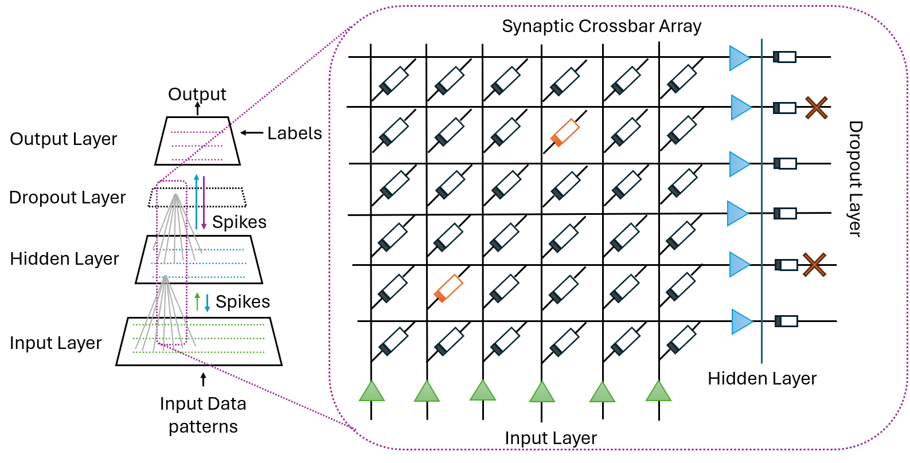
\includegraphics[width=0.95\textwidth]{Chapter7/Figs/a.png}}
    \caption[Proposed Neuromorphic architecture with homeostasis dropout]{Proposed Neuromorphic architecture with homeostasis dropout. A fully connected spiking neural network featuring input, hidden, dropout and output layers of spiking neurons, with synaptic connections illustrated for one neuron in the input and hidden layers. A portion of the neural network implemented with an RRAM crossbar memory array and neuron columns and rows, incorporating a homeostasis dropout layer for broken or overactive devices (red).}
    \label{fig:7a}
\end{figure*}
    

\noindent The described homeostasis mechanism can be applied as a dropout regularization layer in spiking neural networks (SNNs) \cite{stoffel2024spiking}. The synapse's conductance adjusts according to the firing frequency of the presynaptic neuron by utilising a non-monotonic response to the input firing rate. At lower firing rates, the conductance is higher, while at higher frequencies, it decreases, promoting synaptic depression. This behavior enables the system to suppress the influence of overactive or faulty neurons by adapting the conductance individually for each synapse. The advantage of this approach lies in its simplicity, as it does not require the presynaptic neuron to produce pulses of opposite polarity nor access to the postsynaptic side, thereby simplifying circuit design and enhancing regularization in SNNs. \\

\noindent In order to implement dropout regularization in spiking neural networks (SNNs), a homeostasis mechanism is employed that adjusts the synaptic conductance based on the input neuron’s firing rate \cite{kim2021spiking}. The synaptic conductance \( G \) is modeled as a function of the firing rate \( r_{\text{in}} \) of the presynaptic neuron. Specifically, the steady-state conductance \( G_{\text{steady}} \) is defined as a non-monotonic function of \( r_{\text{in}} \), where the conductance increases at lower firing rates and decreases when the firing rate surpasses a threshold, thereby inducing synaptic depression. The functional relationship between the firing rate and synaptic conductance is given by the following:
\begin{equation}
G_{\text{steady}} = \frac{G_{\text{max}}}{1 + \left(\frac{r_{\text{in}}}{r_{\text{threshold}}}\right)^n} \label{eq:7.1}
\end{equation}


\noindent Here, \( G_{\text{max}} \) represents the maximum conductance, \( r_{\text{threshold}} \) is the firing rate at which depression begins, and \( n \) controls the sharpness of the transition. This model allows for the suppression of synapses connected to neurons exhibiting high-frequency activity, effectively implementing a form of dropout. The output current \( I_{\text{out}} \) from the synapse is then determined by the product of the synaptic conductance \( G_{\text{steady}} \) and the input voltage \( V_{\text{in}} \):
\begin{equation}
I_{\text{out}} = G_{\text{steady}} \cdot V_{\text{in}} \label{eq:7.2}
\end{equation}

\noindent This dynamic adjustment of conductance provides a mechanism for selectively reducing the influence of overactive neurons during training, akin to traditional dropout in conventional neural networks. By modulating synaptic conductance based on firing rates, this approach ensures that only relevant connections are active, improving the network's robustness and preventing overfitting. \\

\begin{figure*}[!t]
    \centerline{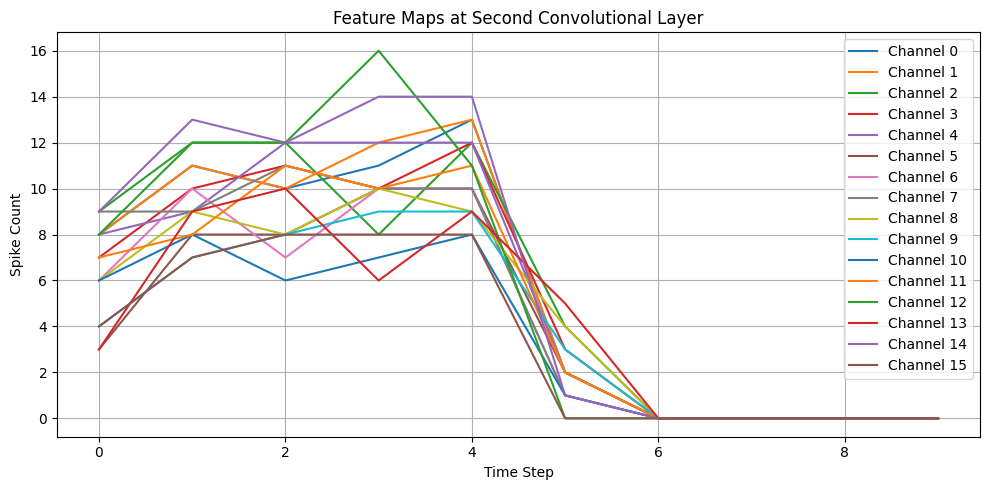
\includegraphics[width=0.8\textwidth]{Chapter7/Figs/b.png}}
    \caption[Feature maps at the second convolutional layer.]{Feature maps at the second convolutional layer. The plot demonstrates the suppression of simulated hyperactive neurons in a memristive spiking neural network for a convolutional layer with 16 hidden channels, at a threshold of 5 time steps.}
    \label{fig:7b}
\end{figure*}

\noindent The homeostasis-dropout method utilizes the time-step mechanism in SNN by focusing on the outputs from a window of the latest selected time steps instead of averaging across all steps. By dynamically adjusting synaptic conductance based on firing rates, this approach identifies a time-local window of significant activity, enabling selective suppression of overactive neurons. This not only reduces computational costs by avoiding redundant evaluations but also enhances robustness and prevents overfitting by emphasizing the most relevant temporal features during training and inference.

\section[Practical Applications]{Practical Applications}

\subsection{Dropout Improvement}


\noindent A two-layer memristive Spiking Neural Network (MSNN) was designed to evaluate its performance on the MNIST dataset, which was converted into spike trains.The network, with a batch size of 64, was trained on 60,000 samples and tested on 10,000. The network contains 100 hidden neurons with Leaky Integrate-and-Fire (LIF) activation and a 10-neuron output layer.Synaptic weights were initialised randomly and updated during training over 1 epoch, with a learning rate of 5e-4 and 50 steps per epoch for 20 epochs.A homeostasis mechanism temporarily disables neurons with excessive spike activity to maintain stable dynamics.\\ 

\noindent The enhanced model, Memristive Convolutional Spiking Neural Network (MCSNN), incorporates convolutional layers to extract more complex features. The MCSNN includes a first convolutional layer with 12 filters using a 5x5 kernel, followed by 2x2 pooling, and a second convolutional layer with 64 filters, also followed by 2x2 pooling. The final layer is a memristive fully connected layer with 10 output neurons.The MCSNN, like the MSNN, uses LIF activation and a digital implementation for compatibility with existing hardware.\\

\noindent Both models are trained with the same hyperparameters, and the cross-entropy loss function from PyTorch is used for training, automatically managing softmax activation of the output layer.The architecture also incorporates kernel density estimation (KDE) to simulate the probabilistic nature of memristor failures and device-to-device variations, and most importantly to observe homeostasis.\\

\begin{figure*}[!t]
    \centerline{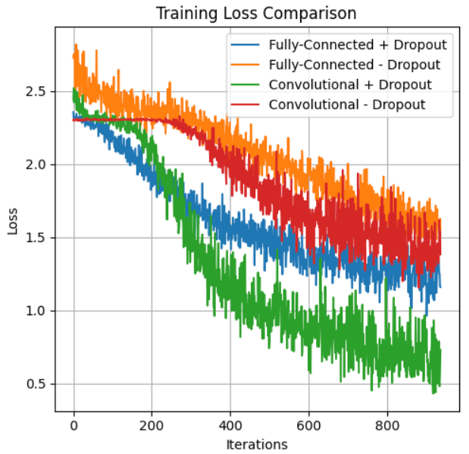
\includegraphics[width=0.6\textwidth]{Chapter7/Figs/c.png}}
    \caption[Training loss curve for standard and memristive schemes when exposed to I-V nonlinearities]{Training loss curve for standard and memristive schemes when exposed to I-V nonlinearities. The loss curves are noisy due to the tracking of losses at every iteration, rather than averaging across multiple iterations.}
    \label{fig:7c}
\end{figure*}


\noindent The training results demonstrate the impact of homeostasis dropout under simulated memristor failures and device-to-device variations at 50\%. Training curves for the MNIST dataset (Fig.\ref{fig:7c}) illustrate the differences between models with and without dropout, with dropout-enhanced models achieving lower loss and outperforming models with simulated faulty devices, particularly in convolutional architectures. \\

\begin{figure*}[!t]
    \centerline{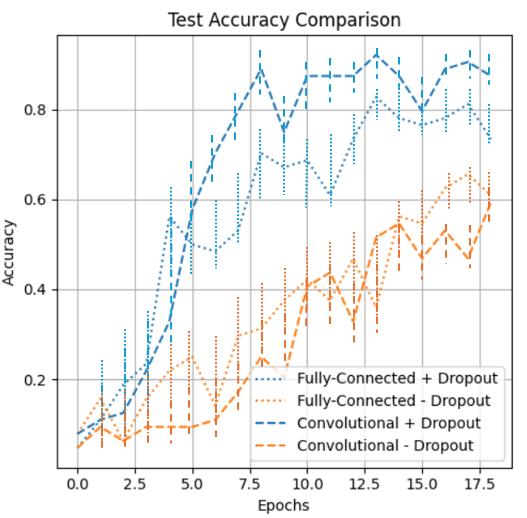
\includegraphics[width=0.6\textwidth]{Chapter7/Figs/d.png}}
    \caption[Training accuracy curve for standard and memristive schemes when exposed to I-V nonlinearities]{Training accuracy curve for standard and memristive schemes when exposed to I-V nonlinearities. Comparison of different spiking neural network performance when implemented with I-V nonlinearities from a single training run.}
    \label{fig:7d}
\end{figure*}
    
\noindent Figure\ref{fig:7d} compares accuracies between SNN and CSNN models, with dropout-improved versions reaching 80-90\%, while models with overactive neurons stabilized at ~60\% after 20 epochs. To address the high variability of non-idealities, which were nondeterministic, five networks were trained for each separate configuration. The results are summarised in table \ref{table:7a}, which demonstrates the efficacy of dropout in mitigating variability and improving performance in SNNs. \\

\begin{table}[!t]
    \caption{Model Accuracy for different SNN configurations}
    \begin{center}
    \begin{tabular}{|c|c|c|}
    \hline
    Model Accuracy  & Homeostasis Dropout & Memristor Failures \\ \hline
    Fully-Connected & $83.37 \pm 3.41 \%$  & $61.54 \pm 4.86 \%$ \\ \hline
    Convolutional   & $91.14 \pm 2.36 \%$  & $65.21 \pm 5.19 \%$  \\ \hline
    \end{tabular}
    \label{table:7a}
    \end{center}
    \vspace*{-\baselineskip}
\end{table}


\noindent In SNN, the membrane potential determines the likelihood of spike emission. During training, the membrane potential is used to compute the loss by comparing the output spike train to the target. When the potential exceeds a threshold, a spike is generated, signaling the neuron to "fire". This is where the homeostasis mechanism applies, as it adjusts synaptic conductance based on the input firing rates. Since the homeostasis regulates spike dynamics instead of direct membrane potential calculation, it acts as a regularization mechanism, modulating synaptic activity. The non-monotonic conductance model mimics biological synaptic plasticity, balancing excitation and inhibition. This balance improves generalization by preventing overfitting, akin to traditional dropout in deep learning.\\

\noindent The subthreshold regime enhances energy efficiency by minimizing current draw, a crucial advantage for edge AI applications. However, its inherently narrow resistance range compromises resilience to voltage noise, increasing susceptibility to errors in large-scale implementations. In complex SNNs, accumulated variations from device non-idealities—such as stochastic switching and drift—can compound over time, degrading overall performance. \\

\begin{figure*}[!t]
    \centerline{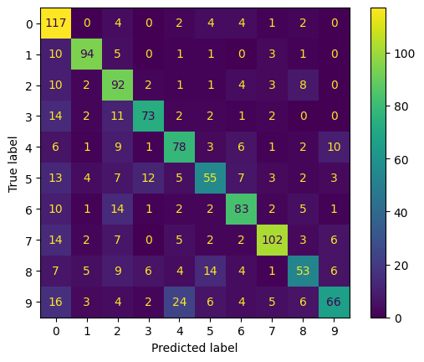
\includegraphics[width=0.6\textwidth]{Chapter7/Figs/e.png}}
    \caption[Confusion matrix of convolutional homeostasis model.]{Confusion matrix for successfully learned MNIST features during validation of convolutional homeostasis model.}
    \label{fig:7e}
\end{figure*}

\noindent While compensation strategies like adaptive learning rules or redundancy help mitigate these effects, they introduce computational overhead that may hinder real-time processing. Furthermore, fabrication inconsistencies can lead to deviations not fully captured by existing models, necessitating further optimization. Achieving both efficiency and robustness remains critical for scaling memristor-based neuromorphic systems in practical deployments.


\subsection{Biosignal Processing}

Biosignals such as Electroencephalogram (EEG) and magnetoencephalogram (MEG) signals carry complex, time-sensitive information about brain activity that traditional deep learning models often struggle to efficiently process. Spiking Neural Networks (SNNs), which encode data as discrete spikes, more closely resemble biological neural signaling and offer significant improvements in temporal precision and energy efficiency compared to conventional Artificial Neural Networks (ANNs).\\

\noindent When augmented with convolutional layers, Convolutional SNNs (CSNNs) harness the spatial-temporal feature extraction power of CNNs while maintaining the sparse and event-driven nature of spiking neurons. CSNNs can achieve >99\% accuracy in detecting anticipatory EEG potentials—signaling user intent—in real-time applications such as braking systems, outperforming standard CNNs and other architectures \cite{lutes2024convolutional}. Similarly CSNNs applied to EEG-based stress detection achieve 98.7\% accuracy, highlighting their robustness and energy-conscious performance \cite{Joshi2025-sa}. \\

\noindent Nevertheless, the implementation of large-scale, low-power SNNs on conventional hardware remains challenging. Memristive hardware has been identified as a potentially effective solution to this issue. The deployment of synaptic weights directly within the fabric of crossbar arrays enables efficient native in-memory computing. This combination of temporal fidelity through event-driven spiking dynamics, energy-efficient spatial feature extraction via convolutional architectures, and ultra-low-power, compact hardware realisation enabled by in-memory memristive technologies represents a significant advance in the field.\\

\noindent Collectively, these characteristics position memristive CSNNs as a potent solution for real-time, on-device biosignal applications, rendering them particularly well-suited for portable, battery-sensitive settings such as brain-computer interfaces, stress monitoring, and ambulatory neurological diagnostics.\\

\noindent To begin, EEG and MEG data were acquired at the MGH/HMS/MIT Athinoula A. Martinos Center for Biomedical Imaging using the Neuromag Vectorview system \cite{Gramfort2020-jm}. EEG recordings were obtained through a 60-channel electrode cap that was synchronized with the MEG system, allowing for simultaneous acquisition of electrophysiological signals from the scalp and magnetic field changes associated with neuronal activity. Structural MRI data for the subject were collected separately using a Siemens 1.5 T Sonata scanner with a magnetization-prepared rapid acquisition gradient-echo (MPRAGE) sequence, providing high-resolution anatomical images suitable for source localization and co-registration with EEG/MEG data.\\

\noindent During the experiment, subjects were exposed to a sequence of stimuli consisting of visual and auditory inputs. Specifically, checkerboard patterns were displayed in either the left or right visual field, and tones were delivered to either the left or right ear. These stimuli were presented at regular intervals of 750 ms. Additionally, at unpredictable intervals, a smiley face appeared at the center of the screen, serving as a visual target to which the participant was instructed to respond by pressing a button with the right index finger as quickly as possible.\\

\noindent Each type of stimulus and response was encoded using specific trigger codes: auditory left (LA = 1), auditory right (RA = 2), visual left (LV = 3), visual right (RV = 4), smiley face (smiley = 5), and button press (button = 32). These trigger events were embedded into the EEG/MEG recordings to enable precise epoching and event-related analysis.\\

\noindent In order to preprocess this data using the MNE-Python library \cite{gramfort2014mne}, the raw EEG and MEG recordings are first loaded, then event triggers are extracted, which identifies the timestamps and codes of all stimulus and response events. The data is then subjected to band-pass filtering, a process that serves to remove noise and artefacts. The selection of appropriate low and high cut-off frequencies is typically undertaken at this stage (e.g., 1–40 Hz). Epochs are created around each event, specifying the time window relative to each stimulus onset (e.g., -0.2 to 0.5 seconds).\\

\noindent Baseline correction is typically implemented within a pre-stimulus window (e.g., -0.2 to 0 s) with the objective of reducing drift and enhancing signal clarity. Furthermore, artifact rejection methods such as Independent Component Analysis (ICA) were employed to remove eye-blink or muscle-related artifacts. The preprocessed epochs can subsequently be utilised for further analysis, including event-related potential (ERP) averaging, time-frequency decomposition, and source localisation.\\

\section[Summary]{Summary}

In the future, SNNs could be adapted as spiking autoencoders, benefiting from their ability to efficiently encode and decode temporal and spatial patterns. This could lead to significant advancements in data compression and anomaly detection. Furthermore, SNNs hold promise in bio-signal processing applications, where their biologically inspired architecture can handle complex signals such as electroencephalograms (EEGs) or electromyograms (EMGs). Future studies should explore these applications, integrating SNNs with biosignal data or advanced sensors, and enhancing robustness against device non-idealities for real-time biosignal processing.\\
